\subsubsection{03.04.15}
\begin{enumerate}
	
	\item The time of beginning and ending of the meeting: 16:00 - 21:30.
	
	\item Purposes of the meeting: 
	\begin{enumerate}
		
		\item Investigate about causes of extra friction in the lift and eliminate them.
		
	\end{enumerate}

	\item Work that has been done:
	\begin{enumerate}
		
		\item Today we did a research to find out about obstacles for moving of the slats. There was one problem: the distance between inside pairs of slats was too wide and caused a lot of friction. To solve this problem, we shortened the ribs and axles, which fixed pairs of rails and adjusted the width of both three elements of the lift. The movement of all the pairs of slats became easier, so now we won't waste power of motor on friction. Now, when the lift is improved, we can try to use blocks with cable instead of belt for lifting.
        \begin{figure}[H]
	  	  \begin{minipage}[h]{0.2\linewidth}
	  	    \center  
	  	  \end{minipage}
	  	  \begin{minipage}[h]{0.6\linewidth}
	  		\center{
\includegraphics[scale=0.3]{days/03.04.15/images/01}}
	  		\caption{Bursting slats before the improvement}
	  	  \end{minipage}
	   \end{figure}
	   
	   \item In addition, today we held new wire for servos on the lift. This wire was made of standard ones and stregthened by the insulating tape.
	   \begin{figure}[H]
	   	\begin{minipage}[h]{0.2\linewidth}
	   		\center  
	   	\end{minipage}
	   	\begin{minipage}[h]{0.6\linewidth}
	   		\center{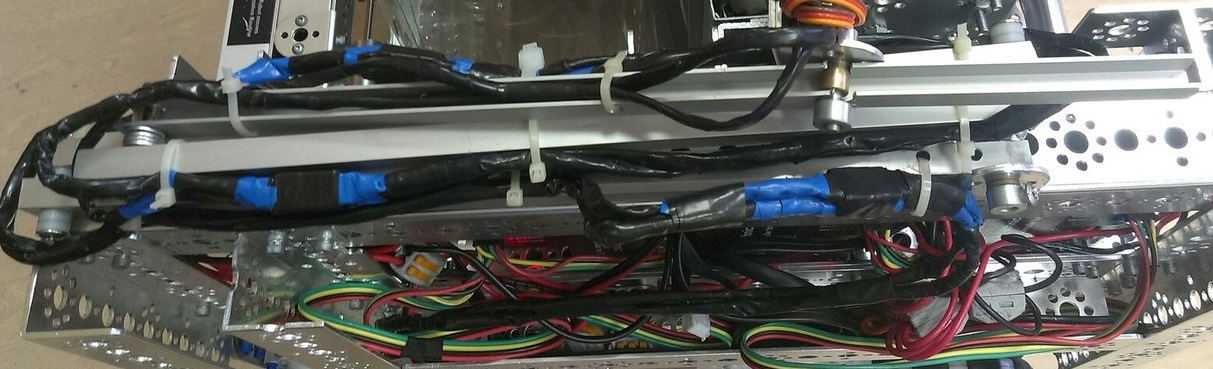
\includegraphics[scale=0.3]{days/03.04.15/images/02}}
	   		\caption{New wire}
	   	\end{minipage}
	   \end{figure}

	\end{enumerate}
	
	\item Results:
	\begin{enumerate}
		
		\item All problems with extra friction in the lift are solved.
		
	\end{enumerate}
	
	\item Tasks for the next meetings:
	\begin{enumerate}
		
		\item Install blocks to the lift and compare its efficiency with the belt.
		
		\item Install AndyMark motors to the lift.
			
	\end{enumerate}
\end{enumerate}
\fillpage
